%----------------------------------------------------------------------------------------
%	PACKAGES AND OTHER DOCUMENT CONFIGURATIONS
%----------------------------------------------------------------------------------------

\documentclass{tufte-book} % Use the tufte-book class which in turn uses the tufte-common class

% \hypersetup{colorlinks} % Comment this line if you don't wish to have colored links

\usepackage{microtype} % Improves character and word spacing

\usepackage{lipsum} % Inserts dummy text

\usepackage{booktabs} % Better horizontal rules in tables

\usepackage{graphicx} % Needed to insert images into the document
\graphicspath{{graphics/}} % Sets the default location of pictures
\setkeys{Gin}{width=\linewidth,totalheight=\textheight,keepaspectratio} % Improves figure scaling

\usepackage{fancyvrb} % Allows customization of verbatim environments
\fvset{fontsize=\normalsize} % The font size of all verbatim text can be changed here

\newcommand{\hangp}[1]{\makebox[0pt][r]{(}#1\makebox[0pt][l]{)}} % New command to create parentheses around text in tables which take up no horizontal space - this improves column spacing
\newcommand{\hangstar}{\makebox[0pt][l]{*}} % New command to create asterisks in tables which take up no horizontal space - this improves column spacing

\usepackage{xspace} % Used for printing a trailing space better than using a tilde (~) using the \xspace command

\newcommand{\monthyear}{\ifcase\month\or January\or February\or March\or April\or May\or June\or July\or August\or September\or October\or November\or December\fi\space\number\year} % A command to print the current month and year

\newcommand{\openepigraph}[2]{ % This block sets up a command for printing an epigraph with 2 arguments - the quote and the author
\begin{fullwidth}
\sffamily\large
\begin{doublespace}
\noindent\allcaps{#1}\\ % The quote
\noindent\allcaps{#2} % The author
\end{doublespace}
\end{fullwidth}
}

\newcommand{\blankpage}{\newpage\hbox{}\thispagestyle{empty}\newpage} % Command to insert a blank page

\usepackage{units} % Used for printing standard units

\newcommand{\hlred}[1]{\textcolor{Maroon}{#1}} % Print text in maroon
\newcommand{\hangleft}[1]{\makebox[0pt][r]{#1}} % Used for printing commands in the index, moves the slash left so the command name aligns with the rest of the text in the index
\newcommand{\hairsp}{\hspace{1pt}} % Command to print a very short space
\newcommand{\ie}{\textit{i.\hairsp{}e.}\xspace} % Command to print i.e.
\newcommand{\eg}{\textit{e.\hairsp{}g.}\xspace} % Command to print e.g.
\newcommand{\na}{\quad--} % Used in tables for N/A cells
\newcommand{\measure}[3]{#1/#2$\times$\unit[#3]{pc}} % Typesets the font size, leading, and measure in the form of: 10/12x26 pc.
\newcommand{\tuftebs}{\symbol{'134}} % Command to print a backslash in tt type in OT1/T1

\providecommand{\XeLaTeX}{X\lower.5ex\hbox{\kern-0.15em\reflectbox{E}}\kern-0.1em\LaTeX}
\newcommand{\tXeLaTeX}{\XeLaTeX\index{XeLaTeX@\protect\XeLaTeX}} % Command to print the XeLaTeX logo while simultaneously adding the position to the index

\newcommand{\doccmdnoindex}[2][]{\texttt{\tuftebs#2}} % Command to print a command in texttt with a backslash of tt type without inserting the command into the index

\newcommand{\doccmddef}[2][]{\hlred{\texttt{\tuftebs#2}}\label{cmd:#2}\ifthenelse{\isempty{#1}} % Command to define a command in red and add it to the index
{ % If no package is specified, add the command to the index
\index{#2 command@\protect\hangleft{\texttt{\tuftebs}}\texttt{#2}}% Command name
}
{ % If a package is also specified as a second argument, add the command and package to the index
\index{#2 command@\protect\hangleft{\texttt{\tuftebs}}\texttt{#2} (\texttt{#1} package)}% Command name
\index{#1 package@\texttt{#1} package}\index{packages!#1@\texttt{#1}}% Package name
}}

\newcommand{\doccmd}[2][]{% Command to define a command and add it to the index
\texttt{\tuftebs#2}%
\ifthenelse{\isempty{#1}}% If no package is specified, add the command to the index
{%
\index{#2 command@\protect\hangleft{\texttt{\tuftebs}}\texttt{#2}}% Command name
}
{%
\index{#2 command@\protect\hangleft{\texttt{\tuftebs}}\texttt{#2} (\texttt{#1} package)}% Command name
\index{#1 package@\texttt{#1} package}\index{packages!#1@\texttt{#1}}% Package name
}}

% A bunch of new commands to print commands, arguments, environments, classes, etc within the text using the correct formatting
\newcommand{\docopt}[1]{\ensuremath{\langle}\textrm{\textit{#1}}\ensuremath{\rangle}}
\newcommand{\docarg}[1]{\textrm{\textit{#1}}}
\newenvironment{docspec}{\begin{quotation}\ttfamily\parskip0pt\parindent0pt\ignorespaces}{\end{quotation}}
\newcommand{\docenv}[1]{\texttt{#1}\index{#1 environment@\texttt{#1} environment}\index{environments!#1@\texttt{#1}}}
\newcommand{\docenvdef}[1]{\hlred{\texttt{#1}}\label{env:#1}\index{#1 environment@\texttt{#1} environment}\index{environments!#1@\texttt{#1}}}
\newcommand{\docpkg}[1]{\texttt{#1}\index{#1 package@\texttt{#1} package}\index{packages!#1@\texttt{#1}}}
\newcommand{\doccls}[1]{\texttt{#1}}
\newcommand{\docclsopt}[1]{\texttt{#1}\index{#1 class option@\texttt{#1} class option}\index{class options!#1@\texttt{#1}}}
\newcommand{\docclsoptdef}[1]{\hlred{\texttt{#1}}\label{clsopt:#1}\index{#1 class option@\texttt{#1} class option}\index{class options!#1@\texttt{#1}}}
\newcommand{\docmsg}[2]{\bigskip\begin{fullwidth}\noindent\ttfamily#1\end{fullwidth}\medskip\par\noindent#2}
\newcommand{\docfilehook}[2]{\texttt{#1}\index{file hooks!#2}\index{#1@\texttt{#1}}}
\newcommand{\doccounter}[1]{\texttt{#1}\index{#1 counter@\texttt{#1} counter}}

\usepackage{makeidx} % Used to generate the index
\makeindex % Generate the index which is printed at the end of the document

% This block contains a number of shortcuts used throughout the book
\newcommand{\vdqi}{\textit{VDQI}\xspace}
\newcommand{\ei}{\textit{EI}\xspace}
\newcommand{\ve}{\textit{VE}\xspace}
\newcommand{\be}{\textit{BE}\xspace}
\newcommand{\VDQI}{\textit{The Visual Display of Quantitative Information}\xspace}
\newcommand{\EI}{\textit{Envisioning Information}\xspace}
\newcommand{\VE}{\textit{Visual Explanations}\xspace}
\newcommand{\BE}{\textit{Beautiful Evidence}\xspace}
\newcommand{\TL}{Tufte-\LaTeX\xspace}

%----------------------------------------------------------------------------------------
%	BOOK META-INFORMATION
%----------------------------------------------------------------------------------------

\title{Beyond Letterboxing: Spatial Interface Patterns for Virtual Reality} % Title of the book

\author[Tobias Bernard]{Tobias\ Bernard} % Author

\publisher{TU Berlin} % Publisher

%----------------------------------------------------------------------------------------

\begin{document}

\frontmatter


%----------------------------------------------------------------------------------------

\maketitlepage % Print the title page

%----------------------------------------------------------------------------------------
%	COPYRIGHT PAGE
%----------------------------------------------------------------------------------------

\newpage
\begin{fullwidth}
~\vfill
\thispagestyle{empty}
\setlength{\parindent}{0pt}
\setlength{\parskip}{\baselineskip}
Copyright \copyright\ \the\year\ \thanklessauthor

\par\smallcaps{Published by \thanklesspublisher}

\par\smallcaps{tufte-latex.googlecode.com}

\par Licensed under the Apache License, Version 2.0 (the ``License''); you may not use this file except in compliance with the License. You may obtain a copy of the License at \url{http://www.apache.org/licenses/LICENSE-2.0}. Unless required by applicable law or agreed to in writing, software distributed under the License is distributed on an \smallcaps{``AS IS'' BASIS, WITHOUT WARRANTIES OR CONDITIONS OF ANY KIND}, either express or implied. See the License for the specific language governing permissions and limitations under the License.\index{license}

\par\textit{First printing, \monthyear}
\end{fullwidth}

%----------------------------------------------------------------------------------------

\tableofcontents % Print the table of contents


\mainmatter

%----------------------------------------------------------------------------------------
%	ABSTRACT
%----------------------------------------------------------------------------------------

% \cleardoublepage
\chapter{Abstract}

Traditionally, graphical user interfaces employ letterboxing in order to display more information than the screen can accomodate at any one time, \ie they employ of a virtual space larger than the screen, which users can interactively navigate. Because users can only see a small part of the letterboxed data space at any given time, it is hard for them to establish a spatial model of the data. This can make interfaces difficult to navigate, especially with large datasets.

Most Virtual Reality applications today employ the same letterboxing patterns as traditional 2D interfaces. It is our hypothesis that \textsc{vr} interfaces could use the possibilities afforded by the 3D environment, in order to improve usability over letterboxing-based approaches.

We will test this hypothesis experimentally by displaying the same dataset (a large set of photos) in different interfaces, some using 2D letterboxing, others using 3D space to display the data. We will record how efficient the different interfaces are to navigate, as well as user satisfaction.



%----------------------------------------------------------------------------------------
%	INTRODUCTION
%----------------------------------------------------------------------------------------

% \cleardoublepage
\chapter{Introduction} % The asterisk leaves out this chapter from the table of contents

When displaying large amounts of information on any medium, whether it's a book, a paper map, or a phone's screen, there are always cases where it isn't possible to show everything at the same time. Strategies for handling this problem are as old as civilization: Ancient scrolls employ a single, linear surface which is then rolled up, books split the information into chunks of similar size and put it on pages which can be stacked, and paper maps are be folded in intricate ways, in order to enable easy navigation in two dimensions (see figure~\ref{fig:falkmap}).

\begin{marginfigure}
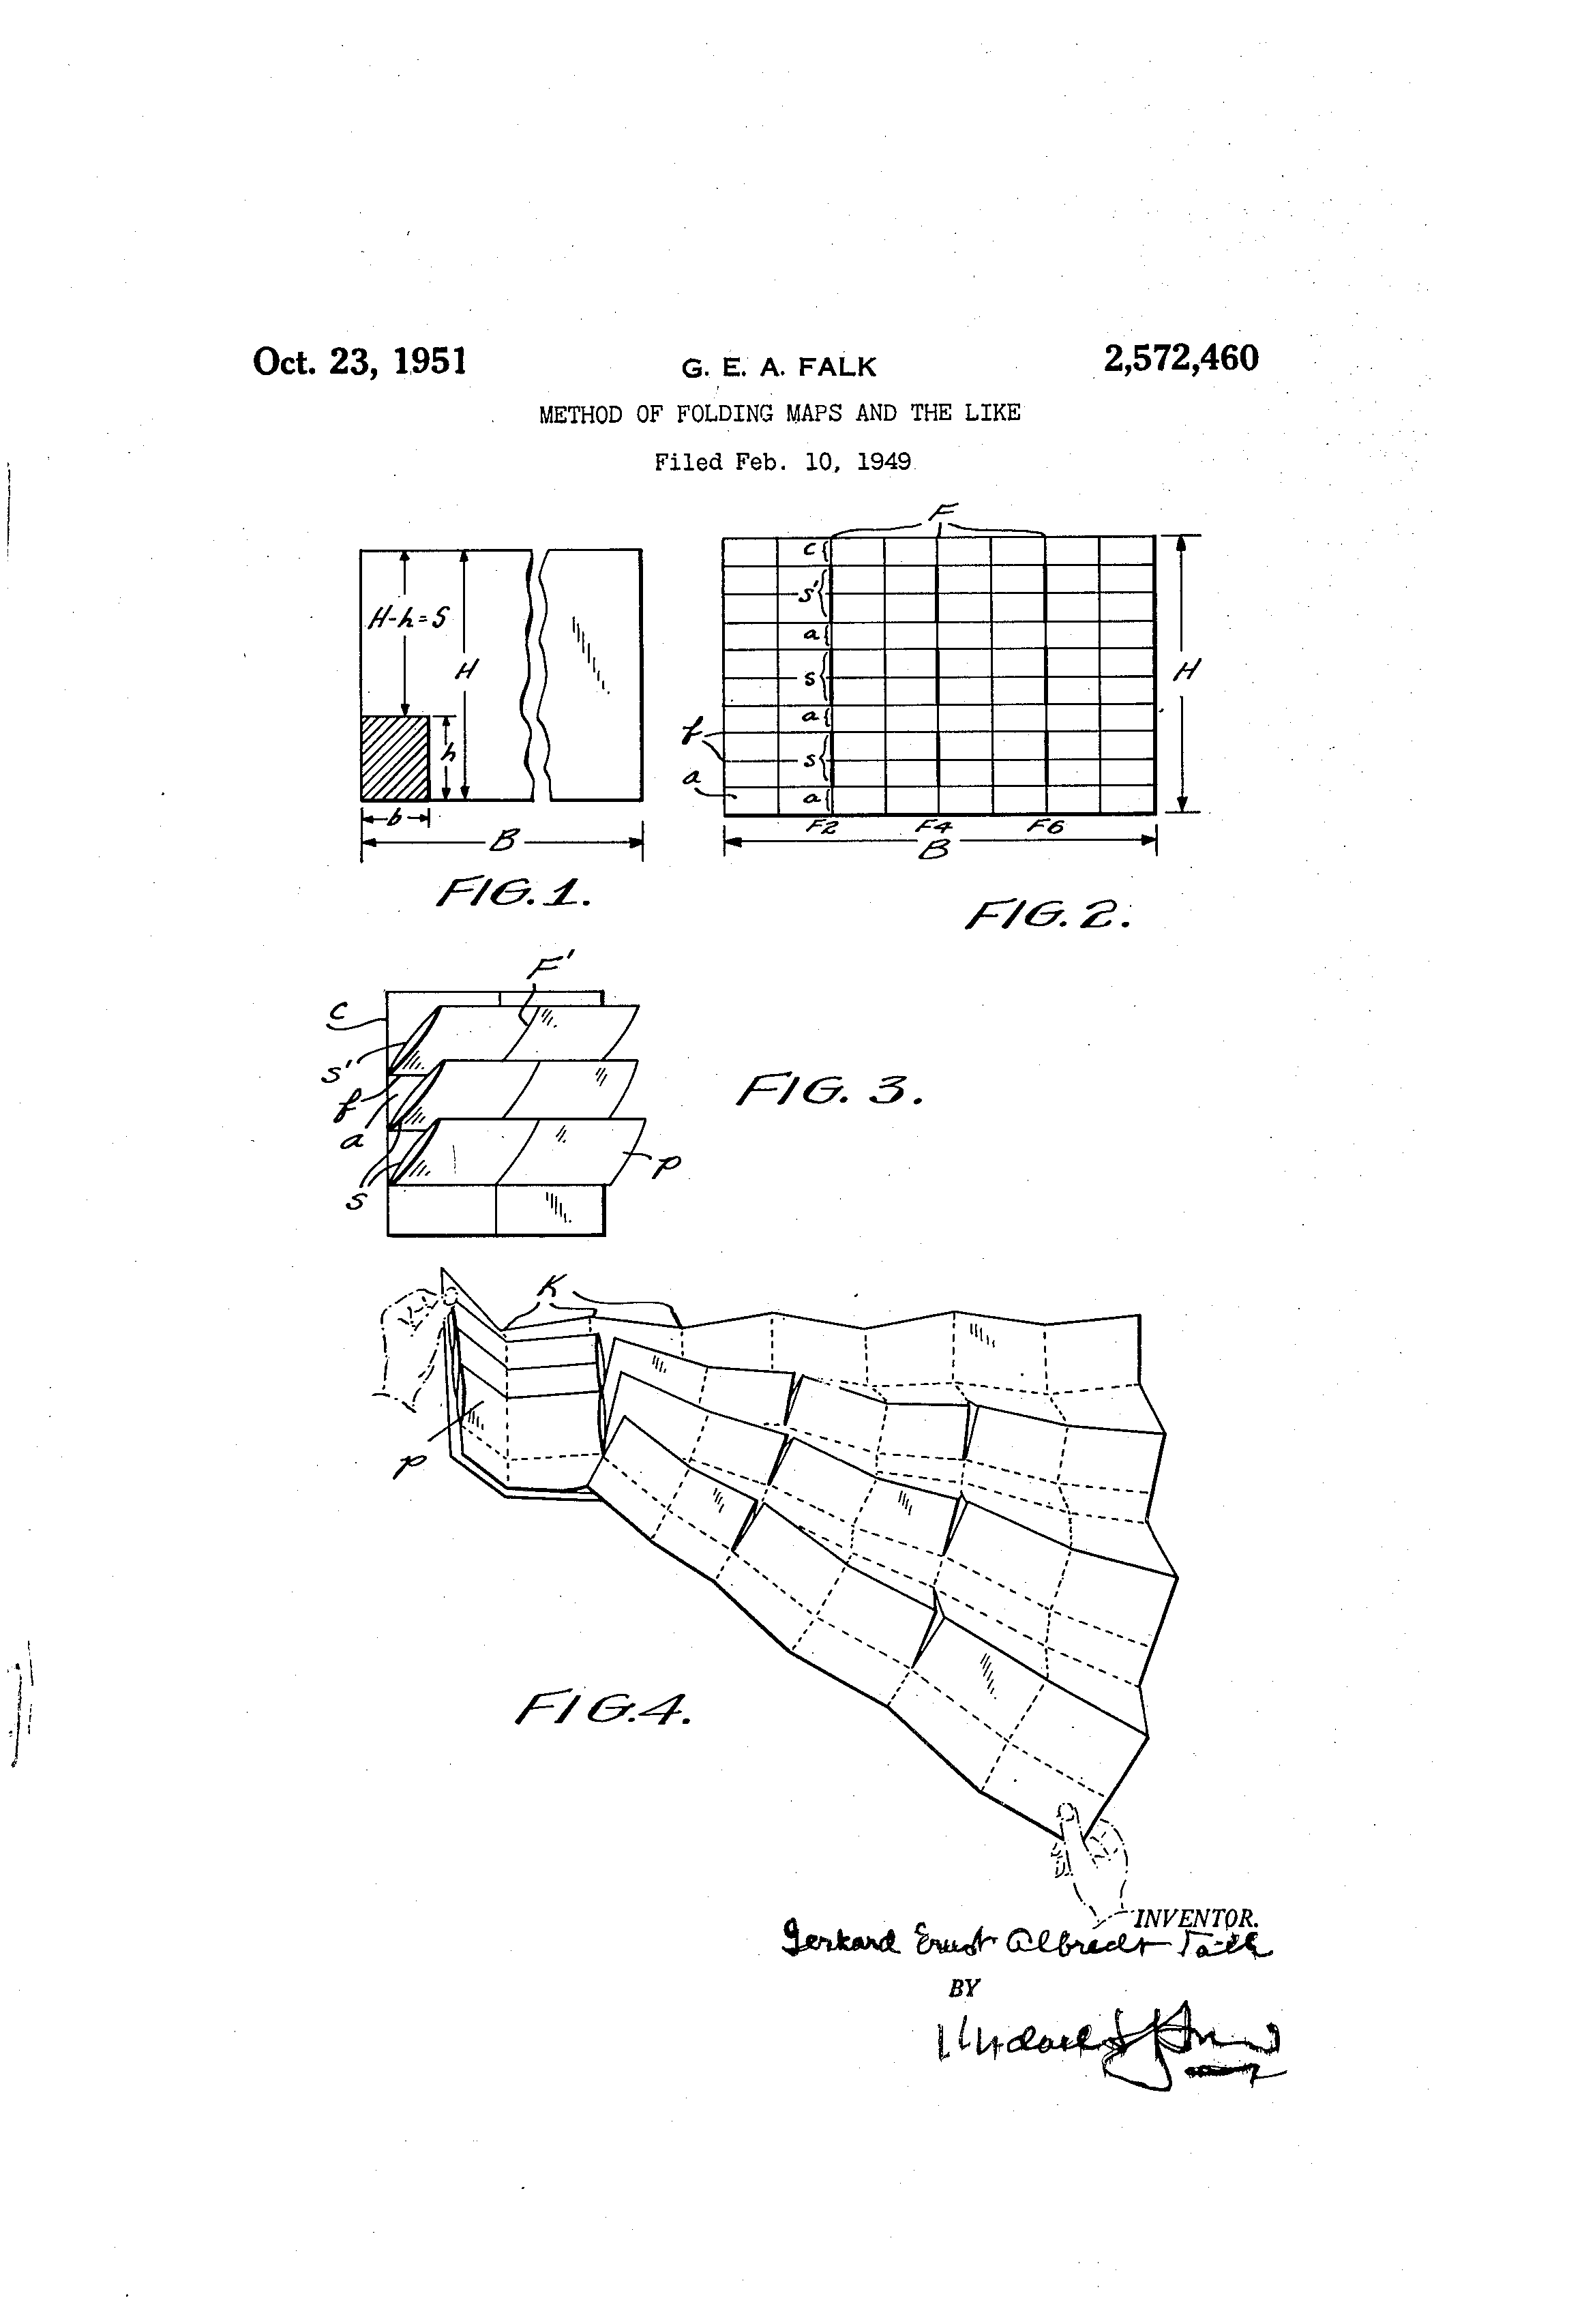
\includegraphics[width=\linewidth]{falk-patent.png}
\caption{US Patent 2572460 \emph{``A United Method for Folding Maps and the Like''}, from 1951 by G. E. A. Falk, describes a technique for folding printed maps in such a way that they can be read without fully unfolding them.}
\label{fig:falkmap}
\end{marginfigure}

In screen-based graphical user interfaces, these cases are usually handled by relying on letterboxing, \ie by employing a virtual space on which all of the information is laid out, and cutting off the content at the edges of the screen. Users can then interactively navigate the virtual space by moving their viewport onto it, \eg by scrolling. This technique works, but it is suboptimal, because it puts the burden of keeping track of the position in the virtual space on the user. Instead of being able to see the entire space they have to rely on their mental model of it.

% It is not ideal, however, because content which is outside the viewport is completely invisible, and the user only has a rudimentary sense of position within the data space.
% they can take up the entire field of vision. However, since this field of vision is not infinitely large, there are still limits to how much data can be viewed at any one time. Since there are no natural boundaries in \textsc{vr}, it does not make sense to use letterboxing to hide the additional information.

Unlike with screens, there are no natural boundaries for Virtual Reality interfaces, because the virtual environment takes up the entire field of vision. Additionally, users can move around in this environment while using an application. This presents the opportunity to use this larger space, as well as the third dimension, in the design of user interfaces.

\begin{figure}
  \includegraphics{pinc2.jpg}
  \caption{Mockup of a Virtual Reality interface covering the entire field of vision (hellopinc.com)}
  \label{fig:noboundaries}
\end{figure}

However, there are currently very few real-world examples of this kind of spatial interface in \textsc{vr}. Most applications are either games or novelty apps such as 3D drawing programs, likely because the 1080p resolution on the current generation of headsets is far too low for most productivity applications.
The interfaces with some complexity that do exist tend to mimic 2D interface patterns and employ letterboxing, often with little or no animations.

\begin{figure}
  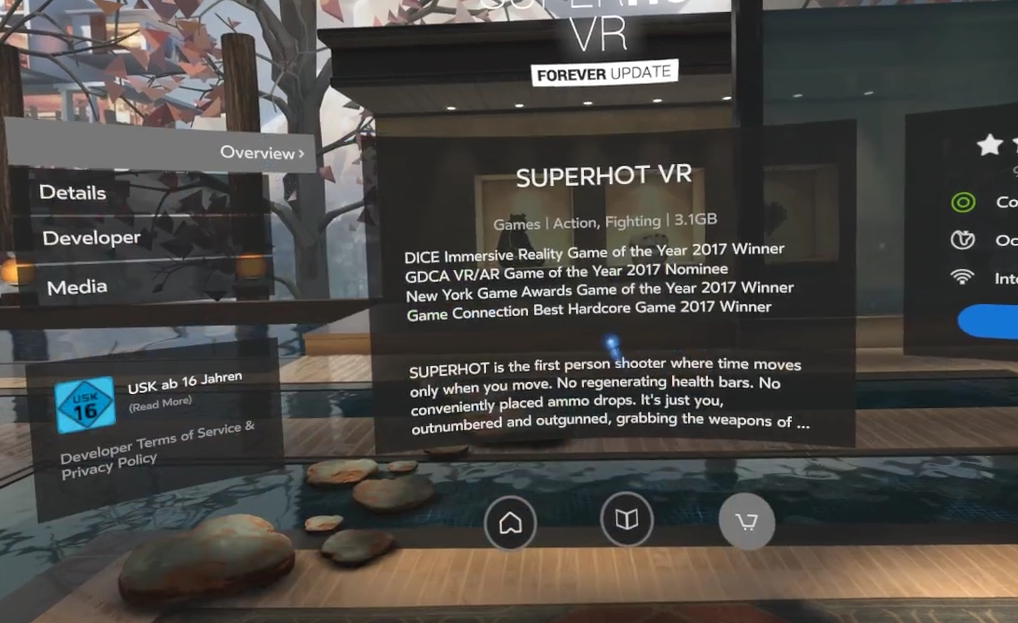
\includegraphics{superhot.png}
  \caption{Application detail page in the Oculus Home store. Clicking the sections on the left changes the content of the center column with a fade animation.}
  \label{fig:superhot}
\end{figure}


In this study we explore spatial interfaces which enable the presentation and navigation of large data sets using the unique possibilities that 3D space affords. For example, instead of disappearing outside the viewport, list items can stack up on top of a list, shrink to a smaller size, or be arranged in a grid.

\begin{marginfigure}
  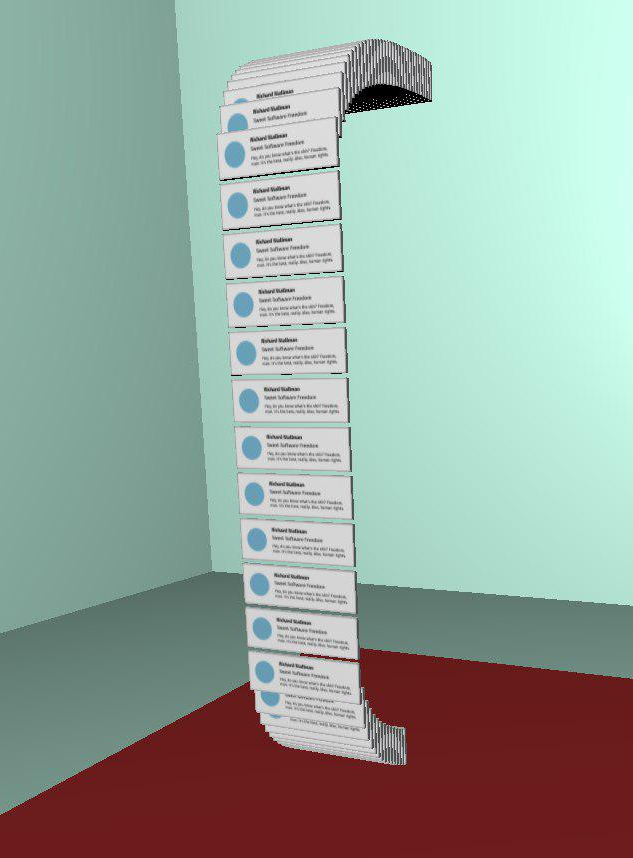
\includegraphics[width=\linewidth]{email.png}
  \caption{Prototype of a list interface which stacks overflowing cards in the z-dimension.}
  \label{fig:email}
\end{marginfigure}

\subsection{Reserach Question}
The primary research question is whether spatial interfaces can improve the usability of \textsc{vr} applications compared to letterboxing. Additionally, we are interested in the advantages and disadvantages of different spatial approaches.

To answer this question we will build a number of different interfaces displaying the same data, some of them spatial, some employing letterboxing. We will then measure how efficient they are to navigate for our test subjects. In addition we will assess the hedonic qualities of the interfaces using a questionnaire.

\subsection{Contributions}
We will develop and evaluate general-purpose patterns for displaying and navigating large amounts of information in \textsc{vr}, which can be used by others building information-dense \textsc{vr} applications in the future. Some of our work may be applicable to 2D interfaces trying to avoid the negative effects of letterboxing as well.

\subsection{Outline}

.........


%----------------------------------------------------------------------------------------
%	RELATED WORK
%----------------------------------------------------------------------------------------

\chapter{Related Work}
\label{ch:related-work}

Related work.........


%----------------------------------------------------------------------------------------
%	PROTOTYPES
%----------------------------------------------------------------------------------------

\chapter{Prototypes}
\label{ch:prototypes}

\section{Technology}
The \textsc{VR} ecosystem is currently (mid 2017) still in its infancy. We experimented with the Oculus Rift \textsc{CV1} and the \textsc{HTC} Vive, both released in early 2016, and tested the headset and controller hardware, software ecosystem, and developer tools.

The installation and setup are very cumbersome for both headsets, especially on the software side, where we encountered many glitches, bugs, and usability problems.

The biggest issue with both headsets is the very low resolution, as both only have a resolution of 1080x1200 per eye. This means that text needs to be either very big, or very close to be legible, and makes any kind of information-dense application impossible. This is exemplified by the fact that the visual entropy of most apps is roughly that of a smartphone, and likely the reason why there are currently only a handful of non-trivial, non-game applications available on both the Oculus store and Steam.

Both headset do room scale tracking relatively well, but we found the Vive tracking to be more reliable, likely due to its trackers being mounted on the walls. Walking around in the roughly 2x2m space feels natural, but the limitations of being able to move only within such a small space quickly become clear in scenarios like games with open-world environments, where it means that teleporting has to be the primary means of movement.

\section{Development}
We developed our prototypes in WebVR using Mozilla's A-Frame Framework. A-Frame is a Javascript library which enables building VR experiences using declarative components directly in HTML. It runs completely standalone in the browser, and can be used with other Javascript libraries and standard web tooling. Though there are sometimes performance and stability issues due to WebVR support in browsers still being experimental, the quality of the experiences is more or less on par with native VR for simple applications.

\section{Prototype 1: Stacked List}
This prototype uses z-depth to stack invisible items behind the visible ones at both ends of a list. The content of these stacked items is not visible, but their presence shows how many items there are both above and below the current position in the list, thereby intuitively communicating this position to the user, without relying on external indicators (\eg scrollbars).

\section{Prototype 2: Elevator}


%----------------------------------------------------------------------------------------
%	EXPERIMENTS
%----------------------------------------------------------------------------------------

\chapter{Experiments}
\label{ch:experiments}

We will construct a series of Virtual Reality scenes, each using a different approach to display the same data, in oder to compare them effectively. Our implementation will make use of a \textsc{vr} headset with positional tracking and two hand controllers to manipulate items in \textsc{vr}. However, due to the low resolution of commercially available \textsc{vr} headsets, we will also evaluate the viability of using a \textsc{cave}, which could potentially provide a higher resolution.

We will evaluate our solutions by running a user study, wherein users navigate our proposed spatial interfaces, as well as a letterboxing-based solution, in order to compare their usability. We will measure efficiency, observe user behavior during the study, and assess user satisfaction using a questionnaire after the experiment.


%----------------------------------------------------------------------------------------
%	RESULTS AND DISCUSSION
%----------------------------------------------------------------------------------------

\chapter{Results and Discussion}
\label{ch:results-and-discussion}


......

%----------------------------------------------------------------------------------------
%	CONCLUSION
%----------------------------------------------------------------------------------------

\chapter{Conclusion}
\label{ch:conclusion}


......

%----------------------------------------------------------------------------------------

\backmatter

%----------------------------------------------------------------------------------------
%	BIBLIOGRAPHY
%----------------------------------------------------------------------------------------

\bibliography{bibliography} % Use the bibliography.bib file for the bibliography
\bibliographystyle{plainnat} % Use the plainnat style of referencing

%----------------------------------------------------------------------------------------

\printindex % Print the index at the very end of the document

\end{document}
